% answers.tex —— 2011 年·山东卷·文科 · 参考答案与详细解析片段
% 由 tools/generate_projects.py 依来源总账自 2011/2011_数学真题_山东文_试题.md + 2011/2011_数学真题_山东文_解析正文.md + 2011/2011_数学真题_山东文_答案要点.md 生成，勿手改（改源 MD 后重跑）


\begin{gktip}
固定源 PDF 只有题面、无答案页，原页未印分值（原页未标）。以下解析与结论均由本库独立推导（非官方答案），并按 600 dpi 原页逐栏复核题面。

【源疑点】第 18 题第（2）问的「2」与第 19 题第（2）问的「$\parallel$」都不在按栏裁切的文字层里（前者略超出栏宽、后者用符号字体），均按 600 dpi 原页图转录，不属原页缺陷。第 11 题原页把两个矩形印在三个命题之后、四个选项之前，本库按体例把图移到选项之后，图内容照原页。第 10 题的（D）在原页是手绘干扰曲线，不对应任何简单解析式。

【图形说明】第 10、11、14、19、21、22 题的图形均依原页重绘，不按比例。第 10 题四个选项由原页矢量路径数字化反解（以原点与 $2\pi$ 刻度相距 $35.61\,\mathrm{pt}$ 定标，即 $1$ 弧度 $=5.6698\,\mathrm{pt}$）：（C）即 $y=\dfrac x2-2\sin x$（拟合残差 $0.008$），（A）为 $y=\dfrac x2-2\cos x$（残差 $0.0014$），（B）为 $y=x-3\sin x$（残差 $0.002$，原页只画到 $|x|\leqslant4$），（D）是原页手绘的干扰曲线（每侧三段三次贝塞尔、两支中心对称），不对应任何简单解析式，重绘时直接使用原页控制点。第 14 题框图、第 19 题四棱台、第 21 题容器、第 22 题椭圆均按原页矢量层逐框、逐棱、逐点实测复刻。
\end{gktip}

\begin{answer}
\gksolhead{1}{}

\textbf{题目}：

设集合 $M=\{x\mid (x+3)(x-2)<0\}$，$N=\{x\mid 1\leqslant x\leqslant 3\}$，则 $M\cap N=$\mbox{（　　）}

（A）$[1,2)$

（B）$[1,2]$

（C）$(2,3]$

（D）$[2,3]$

\Needspace{4\baselineskip}
\textbf{解析}

\Needspace{5\baselineskip}
先解 $M$。$(x+3)(x-2)<0$ 的两根为 $-3$ 与 $2$，二次项系数为正，故解集为两根之间：
\nopagebreak[4]
\[
M=\{x\mid -3<x<2\}=(-3,2).
\]
$N=\{x\mid 1\leqslant x\leqslant 3\}=[1,3]$。求交集时两端点逐个检验：

\begin{itemize}
\item 左端 $1$：$1\in(-3,2)$ 且 $1\in[1,3]$，属于交集，故左端闭合；
\item 右端 $2$：$2\notin(-3,2)$（$M$ 在 $2$ 处开），故右端开。
\end{itemize}

\Needspace{5\baselineskip}
$M$ 的上界 $2$ 小于 $N$ 的上界 $3$，两个区间有重叠，交集非空，故
\nopagebreak[4]
\[
M\cap N=[1,2).
\]

逐项排除：

\begin{itemize}
\item A $[1,2)$ 与计算结果一致；
\item B $[1,2]$ 把 $2$ 收了进去，而 $2\notin M$；
\item C $(2,3]$ 落在 $M$ 之外（$x>2$ 时 $(x+3)(x-2)>0$），且漏掉了 $1\leqslant x\leqslant2$；
\item D $[2,3]$ 同样整段落在 $M$ 之外。
\end{itemize}

选 A。

\gkanswer{答案：A。}

\end{answer}
\begin{answer}
\gksolhead{2}{}

\textbf{题目}：

复数 $z=\dfrac{2-\mathrm i}{2+\mathrm i}$（$\mathrm i$ 为虚数单位）在复平面内对应的点所在的象限为\mbox{（　　）}

（A）第一象限

（B）第二象限

（C）第三象限

（D）第四象限

\Needspace{4\baselineskip}
\textbf{解析}

\Needspace{5\baselineskip}
分子分母同乘分母的共轭 $2-\mathrm i$：
\nopagebreak[4]
\[
z=\frac{2-\mathrm i}{2+\mathrm i}=\frac{(2-\mathrm i)(2-\mathrm i)}{(2+\mathrm i)(2-\mathrm i)}=\frac{(2-\mathrm i)^2}{4+1}.
\]
\Needspace{5\baselineskip}
展开 $(2-\mathrm i)^2=4-4\mathrm i+\mathrm i^2=3-4\mathrm i$，故
\nopagebreak[4]
\[
z=\frac{3-4\mathrm i}{5}=\frac35-\frac45\mathrm i.
\]
实部 $\dfrac35>0$、虚部 $-\dfrac45<0$，对应点 $\left(\dfrac35,-\dfrac45\right)$ 在第四象限。

\Needspace{5\baselineskip}
二次复算：直接验算 $z(2+\mathrm i)=2-\mathrm i$，取 $z=\dfrac35-\dfrac45\mathrm i$，则
\nopagebreak[4]
\[
\left(\frac35-\frac45\mathrm i\right)(2+\mathrm i)=\frac65+\frac35\mathrm i-\frac85\mathrm i-\frac45\mathrm i^2=\frac65-\mathrm i+\frac45=2-\mathrm i,
\]
与题设一致。

逐项排除：A 第一象限要求虚部为正，这里虚部为负；B 第二象限要求实部为负；C 第三象限要求两者皆负，实部实为正；D 与计算结果一致。

选 D。

\gkanswer{答案：D。}

\end{answer}
\begin{answer}
\gksolhead{3}{}

\textbf{题目}：

若点 $(a,9)$ 在函数 $y=3^x$ 的图象上，则 $\tan\dfrac{a\pi}{6}$ 的值为\mbox{（　　）}

（A）$0$

（B）$\dfrac{\sqrt3}{3}$

（C）$1$

（D）$\sqrt3$

\Needspace{4\baselineskip}
\textbf{解析}

$3^a=9=3^2$。指数函数 $y=3^x$ 在 $\mathbf R$ 上严格递增，故 $3^a=3^2$ 当且仅当 $a=2$（唯一性：若 $a>2$ 则 $3^a>9$，若 $a<2$ 则 $3^a<9$）。

\Needspace{5\baselineskip}
于是
\nopagebreak[4]
\[
\tan\frac{a\pi}{6}=\tan\frac{2\pi}{6}=\tan\frac{\pi}{3}=\sqrt3.
\]

代回验证：点 $(2,9)$ 满足 $9=3^2$ 。

逐项排除：A $\tan\dfrac{\pi}{3}\neq0$；B $\dfrac{\sqrt3}{3}=\tan\dfrac{\pi}{6}$，对应 $a=1$，而 $3^1=3\neq9$；C $1=\tan\dfrac{\pi}{4}$，对应 $a=\dfrac32$，$3^{3/2}=3\sqrt3\neq9$；D 与计算结果一致。

选 D。

\gkanswer{答案：D。}

\end{answer}
\begin{answer}
\gksolhead{4}{}

\textbf{题目}：

曲线 $y=x^3+11$ 在点 $P(1,12)$ 处的切线与 $y$ 轴交点的纵坐标是\mbox{（　　）}

（A）$-9$

（B）$-3$

（C）$9$

（D）$15$

\Needspace{4\baselineskip}
\textbf{解析}

\Needspace{5\baselineskip}
设 $y=x^3+11$，则 $y'=3x^2$。在 $x=1$ 处斜率 $k=3\times1^2=3$，切点为 $P(1,12)$（代回：$1^3+11=12$ ）。由点斜式
\nopagebreak[4]
\[
y-12=3(x-1)\ \Longrightarrow\ y=3x+9.
\]
令 $x=0$ 得纵坐标 $y=9$。

代回验证：切线在 $x=1$ 处取 $y=3+9=12$，与切点纵坐标一致；且 $y'|_{x=1}=3$ 等于切线斜率 。

逐项排除：A $-9$ 是把 $x=1$ 代入 $y-12=-3(x-1)$ 的符号错误；B $-3$ 漏了截距平移（误取 $y=3x-6$ 之类的形式）；C 与计算结果一致；D $15$ 误把切点纵坐标 $12$ 与斜率相加。

选 C。

\gkanswer{答案：C。}

\end{answer}
\begin{answer}
\gksolhead{5}{}

\textbf{题目}：

已知 $a$，$b$，$c\in\mathbf R$，命题“若 $a+b+c=3$，则 $a^2+b^2+c^2\geqslant 3$”的否命题是\mbox{（　　）}

（A）若 $a+b+c\neq 3$，则 $a^2+b^2+c^2<3$

（B）若 $a+b+c=3$，则 $a^2+b^2+c^2<3$

（C）若 $a+b+c\neq 3$，则 $a^2+b^2+c^2\geqslant 3$

（D）若 $a^2+b^2+c^2\geqslant 3$，则 $a+b+c=3$

\Needspace{4\baselineskip}
\textbf{解析}

命题「若 $p$ 则 $q$」的否命题是「若 $\lnot p$ 则 $\lnot q$」——条件与结论同时否定，但\textbf{不交换}位置（交换位置并同时否定得到的是逆否命题，与原命题等价，那是另一回事）。

本题 $p$：$a+b+c=3$，$q$：$a^2+b^2+c^2\geqslant3$。故

\begin{itemize}
\item $\lnot p$：$a+b+c\neq3$；
\item $\lnot q$：$a^2+b^2+c^2<3$（「$\geqslant$」的否定是「$<$」，不是「$\leqslant$」）。
\end{itemize}

否命题为：若 $a+b+c\neq3$，则 $a^2+b^2+c^2<3$。

逐项排除：

\begin{itemize}
\item A 与所求一致；
\item B 只否定了结论、没否定条件，既非否命题也非逆命题；
\item C 只否定了条件、结论照抄，是「否条件」而非否命题；
\item D 把条件与结论互换，是逆命题。
\end{itemize}

选 A。

\gkanswer{答案：A。}

\end{answer}
\begin{answer}
\gksolhead{6}{}

\textbf{题目}：

若函数 $f(x)=\sin\omega x$（$\omega>0$）在区间 $\left[0,\dfrac{\pi}{3}\right]$ 上单调递增，在区间 $\left[\dfrac{\pi}{3},\dfrac{\pi}{2}\right]$ 上单调递减，则 $\omega=$\mbox{（　　）}

（A）$\dfrac23$

（B）$\dfrac32$

（C）$2$

（D）$3$

\Needspace{4\baselineskip}
\textbf{解析}

\Needspace{5\baselineskip}
$f(x)=\sin\omega x$（$\omega>0$）的周期为 $\dfrac{2\pi}{\omega}$，在 $x=\dfrac{\pi}{3}$ 处由增转减，说明 $x=\dfrac{\pi}{3}$ 是极大值点：
\nopagebreak[4]
\[
\sin\frac{\omega\pi}{3}=1\ \Longrightarrow\ \frac{\omega\pi}{3}=\frac{\pi}{2}+2k\pi\ (k\in\mathbf Z).
\]
$\omega>0$ 的最小正解（$k=0$）为 $\omega=\dfrac32$。

验证：$\omega=\dfrac32$ 时 $f(x)=\sin\dfrac{3x}{2}$，当 $x\in\left[0,\dfrac{\pi}{3}\right]$ 有 $\dfrac{3x}{2}\in\left[0,\dfrac{\pi}{2}\right]$，$f$ 递增 ；当 $x\in\left[\dfrac{\pi}{3},\dfrac{\pi}{2}\right]$ 有 $\dfrac{3x}{2}\in\left[\dfrac{\pi}{2},\dfrac{3\pi}{4}\right]$，$f$ 递减 （$\dfrac{3\pi}{4}<\pi$，仍在单调递减段内）。

逐项排除：A $\omega=\dfrac23$ 时 $\dfrac{\omega\pi}{3}=\dfrac{2\pi}{9}<\dfrac{\pi}{2}$，$f$ 在 $\left[0,\dfrac{\pi}{3}\right]$ 上仍在递增，没有极大值点；C $\omega=2$ 时 $\dfrac{2\pi}{3}$ 处 $\sin\dfrac{2\pi}{3}=\dfrac{\sqrt3}{2}<1$，$x=\dfrac{\pi}{3}$ 不是极值点；D $\omega=3$ 时 $\sin\pi=0$，$x=\dfrac{\pi}{3}$ 处 $f$ 由正转负，是零点而非极值点。

选 B。

\gkanswer{答案：B。}

\end{answer}
\begin{answer}
\gksolhead{7}{}

\textbf{题目}：

\Needspace{5\baselineskip}
设变量 $x$，$y$ 满足约束条件
\nopagebreak[4]
\[
\begin{cases}
x+2y-5\leqslant 0,\\
x-y-2\leqslant 0,\\
x\geqslant 0,
\end{cases}
\]
则目标函数 $z=2x+3y+1$ 的最大值为\mbox{（　　）}

（A）$11$

（B）$10$

（C）$9$

（D）$8.5$

\Needspace{4\baselineskip}
\textbf{解析}

三条约束依次是 $y\leqslant\dfrac{5-x}{2}$、$y\geqslant x-2$、$x\geqslant0$（题设没有 $y\geqslant0$，可行域不是第一象限的三角形，须由两斜线自行定界）。

由 $x-2\leqslant\dfrac{5-x}{2}$ 得 $2x-4\leqslant5-x$，即 $x\leqslant3$；故 $0\leqslant x\leqslant3$。三个顶点：

\begin{itemize}
\item $x=0$ 与 $y=x-2$ 交于 $(0,-2)$；
\item $x=0$ 与 $y=\dfrac{5-x}{2}$ 交于 $\left(0,\dfrac52\right)$；
\item 两斜线交于 $x=3$、$y=1$，即 $(3,1)$（检验：$3+2\times1=5$ ，$3-1=2$ ）。
\end{itemize}

\Needspace{5\baselineskip}
这是三角形区域。$z=2x+3y+1$ 是线性函数，最值在顶点取到：
\nopagebreak[4]
\[
z\left(0,\frac52\right)=0+\frac{15}{2}+1=\frac{17}{2}=8.5,\qquad
z(0,-2)=0-6+1=-5,\qquad
z(3,1)=6+3+1=10.
\]
最大值 $10$。

代回验证：$(3,1)$ 满足三条约束 $3+2=5\leqslant5$、$3-1=2\leqslant2$、$3\geqslant0$ ；且目标函数沿 $y$ 增大方向系数为正，取到 $y$ 的上界处最大，与顶点比较一致。

逐项排除：A $11$ 取不到——$z=11$ 要求 $2x+3y=10$，$x=0$ 时 $y=\dfrac{10}{3}>\dfrac52$ 已越出上界，沿上边界 $x+2y=5$ 有 $z=\dfrac x2+8.5\leqslant10$；B $10$ 在顶点 $(3,1)$ 取到，与计算结果一致；C $9$ 确实被取到（如 $(1,2)$：$2+6+1=9$），但不是最大值；D $8.5$ 是顶点 $\left(0,\dfrac52\right)$ 处的值，只是次大值。

选 B。

\gkanswer{答案：B。}

\end{answer}
\begin{answer}
\gksolhead{8}{}

\textbf{题目}：

某产品的广告费用 $x$ 与销售额 $y$ 的统计数据如下表：

\begin{center}
\begin{tabular}{lrrrr}
\toprule
广告费用 $x$（万元） & $4$ & $2$ & $3$ & $5$ \\
\midrule
销售额 $y$（万元） & $49$ & $26$ & $39$ & $54$ \\
\bottomrule
\end{tabular}
\end{center}

根据上表可得回归方程 $\hat y=\hat bx+\hat a$ 中的 $\hat b$ 为 $9.4$，据此模型预报广告费用为 $6$ 万元时销售额为\mbox{（　　）}

（A）$63.6$ 万元

（B）$65.5$ 万元

（C）$67.7$ 万元

（D）$72.0$ 万元

\Needspace{4\baselineskip}
\textbf{解析}

\Needspace{5\baselineskip}
先算两个平均数：
\nopagebreak[4]
\[
\bar x=\frac{4+2+3+5}{4}=3.5,\qquad \bar y=\frac{49+26+39+54}{4}=\frac{168}{4}=42.
\]
\Needspace{5\baselineskip}
回归直线过样本中心 $(\bar x,\bar y)$，故
\nopagebreak[4]
\[
\hat a=\bar y-\hat b\bar x=42-9.4\times3.5=42-32.9=9.1.
\]
（顺便核对题给的 $\hat b=9.4$：$\sum(x_i-\bar x)(y_i-\bar y)=0.5\times7+(-1.5)(-16)+(-0.5)(-3)+1.5\times12=3.5+24+1.5+18=47$，$\sum(x_i-\bar x)^2=0.25+2.25+0.25+2.25=5$，$\hat b=\dfrac{47}{5}=9.4$ 。）

\Needspace{5\baselineskip}
$x=6$ 时
\nopagebreak[4]
\[
\hat y=9.4\times6+9.1=56.4+9.1=65.5\ (\text{\text{万元}}).
\]

代回验证：把 $x=3.5$ 代入得 $9.4\times3.5+9.1=42=\bar y$ ，回归直线确实过样本中心。

逐项排除：四项都等于 $9.4\times6+\hat a=56.4+\hat a$，反推各自的 $\hat a$ 为 $7.2$、$9.1$、$11.3$、$15.6$。A 的 $7.2$ 与 C 的 $11.3$ 都是 $\hat a$ 算错（例如漏除样本量、或把 $\bar y$ 与 $\hat b\bar x$ 的次序弄反）；D 的 $15.6$ 相当于把 $6$ 万元直接代进另一种错误的回归式。只有 B 对应正确的 $\hat a=9.1$。

选 B。

\gkanswer{答案：B。}

\end{answer}
\begin{answer}
\gksolhead{9}{}

\textbf{题目}：

设 $M(x_0,y_0)$ 为抛物线 $C:x^2=8y$ 上一点，$F$ 为抛物线 $C$ 的焦点，以 $F$ 为圆心、$|FM|$ 为半径的圆和抛物线 $C$ 的准线相交，则 $y_0$ 的取值范围是\mbox{（　　）}

（A）$(0,2)$

（B）$[0,2]$

（C）$(2,+\infty)$

（D）$[2,+\infty)$

\Needspace{4\baselineskip}
\textbf{解析}

\Needspace{5\baselineskip}
$x^2=8y$ 即 $x^2=2py$，$2p=8$、$p=4$：焦点 $F(0,2)$，准线 $y=-2$。抛物线上点 $M(x_0,y_0)$ 到焦点的距离等于到准线的距离，即
\nopagebreak[4]
\[
|FM|=y_0-(-2)=y_0+2,
\]
且 $y_0\geqslant0$（抛物线开口向上，顶点在原点）。

\Needspace{5\baselineskip}
圆心 $F(0,2)$ 到准线 $y=-2$ 的距离为 $4$。圆与准线相交当且仅当半径\textbf{大于}圆心到直线的距离（等于时相切，只有一个公共点，不算相交）：
\nopagebreak[4]
\[
|FM|>4\ \Longrightarrow\ y_0+2>4\ \Longrightarrow\ y_0>2.
\]
再结合 $y_0\geqslant0$，得 $y_0\in(2,+\infty)$。

代回验证：取 $y_0=2.5$，则 $M(\pm\sqrt{20},2.5)$，半径 $4.5>4$，圆 $x^2+(y-2)^2=20.25$ 与 $y=-2$ 交于 $x^2=20.25-16=4.25$，有两个交点 ；取 $y_0=2$，半径恰为 $4$，圆与准线相切于 $(0,-2)$，只有一个公共点，不符合「相交」。

逐项排除：A $(0,2)$ 里 $y_0<2$ 的部分半径小于 $4$，圆与准线不相交；B $[0,2]$ 整个区间都不相交（$y_0=2$ 只是相切）；D $[2,+\infty)$ 把相切的 $y_0=2$ 也收了进去；C 与计算结果一致。

选 C。

\gkanswer{答案：C。}

\end{answer}
\begin{answer}
\gksolhead{10}{}

\textbf{题目}：

函数 $y=\dfrac x2-2\sin x$ 的图象大致是\mbox{（　　）}

（A）图 A

（B）图 B

（C）图 C

（D）图 D
\nopagebreak[4]
\begin{center}% 2011 年山东卷文科第 10 题：四个选项的函数图象（选项图）。
% 来源 PDF：普通高考/2011/2011山东文.pdf，SHA-256 bf61cf7bb39a3ccfc57735cd2a7ab34387cbfa6bc86a5e7f8246e13292b0e023。
% 原页：第 1 页（A3 三栏）第 2 栏上部，书页码 691。
% 重绘依据：按原页矢量层实测复刻。原点与 2π 刻度相距 35.61pt，故 1 弧度 = 35.61/(2π) = 5.6698pt，
%   下文坐标一律以弧度为单位的无量纲数（4 即 y=4，6.283 即 2π）。
%   四个子图的坐标系同形：x 轴自原点左伸 11.99、右伸 11.36 弧度；y 轴上伸 6.36、下伸 7.00；
%   y 轴在 y=4 处有一个向右的短刻度（长 0.40），x 轴在 x=2π 处有一个向上的短刻度（长 0.40）；
%   文字位置一律取原页字形盒中心（换算成弧度）：y 标签 (-1.13,7.25)、4 标签 (-1.07,3.87)、
%   2π 标签 (6.29,-1.38)、x 标签 (12.05,-0.98)、选项字母 (-14.03,-6.45)；
%   原点 O 的标注位置各图不同且照原页：(A) 在 x 轴上方 (-1.38,1.13)，
%   (B)(C)(D) 都在 x 轴下方约 (-1.37,-1.45)。
%   原页四图都无网格、无虚线。
%   曲线由原页矢量路径数字化反解：(C) 是 y=x/2-2sin x（残差 0.008），即本题正确图象；
%   (A) 是 y=x/2-2cos x（残差 0.0014），在 y 轴上的截距为 -2；
%   (B) 是 y=x-3sin x（残差 0.002），原页只画在 |x|≤4 内；
%   (D) 是原页手绘的干扰曲线，不是解析函数：每侧三段三次贝塞尔，两支关于原点中心对称，
%   振幅随 |x| 增大（x=±1.56 处约 ∓2.14，x=±7 处约 ±4.5），零点在 0、±3.42、±8.8；
%   本图直接使用原页控制点（原页坐标除以 5.6698pt），拓扑与形状照原页。
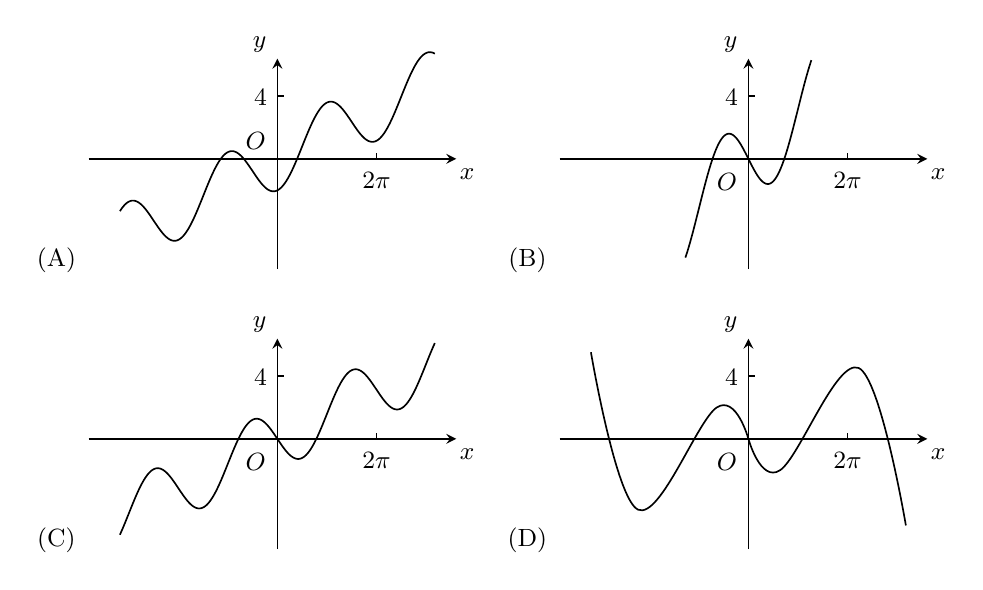
\begin{tikzpicture}[scale=0.20, >=stealth, semithick, font=\small]

  % ===== 四个子图共用的坐标轴（坐标值即原页实测的弧度数；O 的标注各图另放） =====
  \def\axes{
    \draw[->] (-11.99,0) -- (11.36,0);
    \draw[->] (0,-7.00) -- (0,6.36);
    \draw (0,4) -- (0.40,4);
    \draw (6.283,0) -- (6.283,0.40);
    \node at (-1.07,3.87) {$4$};
    \node at (6.29,-1.38) {$2\pi$};
    \node at (12.05,-0.98) {$x$};
    \node at (-1.13,7.25) {$y$};
  }

  % ================= (A) y = x/2 - 2cos x =================
  \begin{scope}
    \axes
    \node at (-1.38,1.13) {$O$};
    \draw[domain=-10:10, samples=300] plot (\x,{\x/2-2*cos(\x r)});
    \node at (-14.03,-6.45) {(A)};
  \end{scope}

  % ================= (B) y = x - 3sin x =================
  \begin{scope}[shift={(29.91,0)}]
    \axes
    \node at (-1.36,-1.45) {$O$};
    \draw[domain=-4:4, samples=200] plot (\x,{\x-3*sin(\x r)});
    \node at (-14.03,-6.45) {(B)};
  \end{scope}

  % ================= (C) y = x/2 - 2sin x =================
  \begin{scope}[shift={(0,-17.78)}]
    \axes
    \node at (-1.38,-1.45) {$O$};
    \draw[domain=-10:10, samples=300] plot (\x,{\x/2-2*sin(\x r)});
    \node at (-14.03,-6.45) {(C)};
  \end{scope}

  % ====== (D) 原页手绘干扰曲线（贝塞尔控制点照原页矢量层） ======
  \begin{scope}[shift={(29.91,-17.78)}]
    \axes
    \node at (-1.36,-1.45) {$O$};
    % 右支：原点 → (2,-2) → (7,4.5) → (10,-5.5)
    \draw (0,0) .. controls (0,0) and (0.767,-2.793) .. (2.000,-2.000)
                .. controls (3.234,-1.207) and (5.590,5.117) .. (7.000,4.500)
                .. controls (8.408,3.883) and (10.000,-5.500) .. (10.000,-5.500);
    % 左支：与右支关于原点中心对称
    \draw (0,0) .. controls (0,0) and (-0.767,2.793) .. (-2.000,2.000)
                .. controls (-3.234,1.207) and (-5.590,-5.117) .. (-7.000,-4.500)
                .. controls (-8.408,-3.883) and (-10.000,5.500) .. (-10.000,5.500);
    \node at (-14.03,-6.45) {(D)};
  \end{scope}

\end{tikzpicture}
\end{center}
\nopagebreak[4]
\Needspace{4\baselineskip}
\textbf{解析}

记 $f(x)=\dfrac x2-2\sin x$。直接算出几个关键量。

\textbf{过原点}：$f(0)=0-0=0$。

\textbf{在原点处的单调性}：$f'(x)=\dfrac12-2\cos x$，$f'(0)=\dfrac12-2=-\dfrac32<0$，图象在原点处下降。

\textbf{奇偶性}：$f(-x)=-\dfrac x2+2\sin x=-f(x)$，为奇函数，图象关于原点中心对称。

\Needspace{5\baselineskip}
\textbf{极值}：$f'(x)=0$ 即 $\cos x=\dfrac14$。在 $(0,2\pi)$ 内有两解 $x_1=\arccos\dfrac14\approx1.32$ 与 $x_2=2\pi-x_1\approx4.96$。$x\in(0,x_1)$ 时 $\cos x>\dfrac14$、$f'<0$；$x\in(x_1,x_2)$ 时 $f'>0$；$x\in(x_2,2\pi)$ 时 $f'<0$。故
\nopagebreak[4]
\[
\begin{aligned}
f(x_1)&=\frac{1.32}{2}-2\times0.9689\approx0.66-1.94=-1.28\ (\text{\text{极小}}),\\
f(x_2)&=\frac{4.96}{2}+2\times0.9689\approx2.48+1.94=4.42\ (\text{\text{极大}}).
\end{aligned}
\]

\textbf{在 $2\pi$ 处}：$f(2\pi)=\pi-0=\pi\approx3.14>0$，而 $f'(2\pi)=\dfrac12-2=-\dfrac32<0$，即曲线在 $2\pi$ 处位于 $x$ 轴上方且正在下降。

按原页矢量路径数字化反解（以原点与 $2\pi$ 刻度定标，残差 $0.008$），（C）正是 $y=\dfrac x2-2\sin x$。

逐项排除：

\begin{itemize}
\item A 在 $y$ 轴上的截距为 $-2$，与 $f(0)=0$ 矛盾（按原页路径反解，它的解析式是 $y=\dfrac x2-2\cos x$，只把 $\sin$ 换成了 $\cos$）；
\item B 过原点、在原点处下降、也是奇函数，但按反解它是 $y=x-3\sin x$：$x$ 的系数是 $1$ 而不是 $\dfrac12$，$\sin$ 的系数是 $3$ 而不是 $2$，故在 $x=1.35$ 处已到 $-1.58$、在 $x=4$ 处已升到 $6.27$，整段图象比 $f$ 陡得多，而原页（B）只画到 $|x|\leqslant4$、没有 $2\pi$ 附近那一段；
\item C 过原点、原点处下降、$x\approx1.32$ 极小 $-1.28$、$x\approx4.96$ 极大 $4.42$、在 $2\pi$ 处 $y=\pi\approx3.14$ 且下降、$x\approx7.60$ 处再取极小 $1.86$，与计算结果逐项吻合；
\item D 虽也过原点，但振幅随 $|x|$ 增大而不减（按反解，$x=\pm1.56$ 处约 $\mp2.14$，$x=\pm7$ 处约 $\pm4.5$），且在 $2\pi$ 附近曲线上行（$x=6.28$ 处约 $4.2$、$x=7$ 处取极大 $4.5$），与 $f(2\pi)=\pi$、$f'(2\pi)=-\dfrac32<0$ 都不符（原页（D）是手绘干扰项，不对应任何简单解析式）。
\end{itemize}

选 C。

\gkanswer{答案：C。}

\end{answer}
\begin{answer}
\gksolhead{11}{}

\textbf{题目}：

如图是长和宽分别相等的两个矩形。给定下列三个命题：① 存在三棱柱，其正（主）视图、俯视图如图；② 存在四棱柱，其正（主）视图、俯视图如图；③ 存在圆柱，其正（主）视图、俯视图如图。其中真命题的个数是\mbox{（　　）}

（A）$3$

（B）$2$

（C）$1$

（D）$0$
\nopagebreak[4]
\begin{center}% 2011 年山东卷文科第 11 题：长和宽分别相等的两个矩形（正（主）视图、俯视图）。
% 来源 PDF：普通高考/2011/2011山东文.pdf，SHA-256 bf61cf7bb39a3ccfc57735cd2a7ab34387cbfa6bc86a5e7f8246e13292b0e023。
% 原页：第 1 页（A3 三栏）第 2 栏中部，书页码 691。
% 重绘依据：照原页——上下两个全等矩形轮廓，原页实测均 56.68pt × 28.34pt，上下间距 21.25pt；
%   上矩形正下方标「正（主）视图」，下矩形正下方标「俯视图」。无阴影、无虚线、无箭头。
% 坐标取原页 pt：X = x_页 − 566.71，Y = 425.05 − y_页。
\begin{tikzpicture}[x=0.05cm, y=0.05cm, semithick, font=\small]
  % 正（主）视图
  \draw (0,49.59) rectangle (56.68,77.93);
  \node[below, inner sep=3pt] at (28.34,49.59) {正（主）视图};
  % 俯视图
  \draw (0,0) rectangle (56.68,28.34);
  \node[below, inner sep=3pt] at (28.34,0) {俯视图};
\end{tikzpicture}
\end{center}
\nopagebreak[4]
\Needspace{4\baselineskip}
\textbf{解析}

两个视图都是「内部没有任何线条的矩形」，且长、宽分别相等。按三视图规则，可见的棱必须画出，故「内部无线条」是强约束：投影方向上不能有棱在轮廓内部留下可见线条，即横截面的各顶点必须在投影方向的两个极端位置（否则中间的棱会投影成轮廓内的直线）。逐个构造。

① \textbf{三棱柱}：取直三棱柱，侧棱水平且垂直于正投影方向（设为左右方向，长 $L$），横截面是直角三角形，两条直角边分别沿竖直方向（长 $h$）与前后方向（长 $w$）。

\begin{itemize}
\item 正视图（沿前后方向投影）：整个柱体是「长 $L$ 的线段 × 截面」的乘积，轮廓为 $L\times h$ 的矩形；三棱柱的三条侧棱分别位于截面的三个顶点，其 $z$ 坐标恰是 $0$、$0$、$h$ 三个极端值，投影全部落在矩形的上下边界上，轮廓内无线条；
\item 俯视图（沿竖直方向投影）：轮廓为 $L\times w$ 的矩形；三条侧棱的 $y$ 坐标恰是 $0$、$w$、$0$，投影全落在矩形的左右边界上，轮廓内同样无线条。
\end{itemize}

两视图的长都是 $L$，宽分别为 $h$ 与 $w$。取 $h=w$（截面为等腰直角三角形）即得长、宽分别相等的两个矩形。① 真。

② \textbf{四棱柱}：取长 $a$、宽（深）$b$、高 $h$ 的长方体。正视图为 $a\times h$，俯视图为 $a\times b$，两者内部都无线条。取 $h=b$ 时两视图是同一个矩形，长、宽分别相等。② 真。

③ \textbf{圆柱}：取轴水平且垂直于正投影方向的圆柱（轴沿前后方向，长 $L$，底面半径 $r$）。正视图是 $L\times2r$ 的矩形（母线投影为上下两条边），俯视图也是 $L\times2r$ 的矩形，两者全等且内部无线条。③ 真。

三个命题都真，真命题个数为 $3$。

逐项排除：B $2$、C $1$、D $0$ 都至少少算了一个可行构造。三个构造的关键分别是：①「侧棱水平 + 截面为等腰直角三角形」，②「高等于宽（深）」，③「轴水平且垂直于正视方向」。若把三棱柱竖放，俯视图是三角形；若把圆柱竖放，俯视图是圆，都不满足。

选 A。

\gkanswer{答案：A。}

\end{answer}
\begin{answer}
\gksolhead{12}{}

\textbf{题目}：

设 $A_1$，$A_2$，$A_3$，$A_4$ 是平面直角坐标系中两两不同的四点，若 $\overrightarrow{A_1A_3}=\lambda\overrightarrow{A_1A_2}$（$\lambda\in\mathbf R$），$\overrightarrow{A_1A_4}=\mu\overrightarrow{A_1A_2}$（$\mu\in\mathbf R$），且 $\dfrac1\lambda+\dfrac1\mu=2$，则称 $A_3$，$A_4$ 调和分割 $A_1$，$A_2$。已知点 $C(c,0)$，$D(d,0)$（$c$，$d\in\mathbf R$）调和分割点 $A(0,0)$，$B(1,0)$，则下面说法正确的是\mbox{（　　）}

（A）$C$ 可能是线段 $AB$ 的中点

（B）$D$ 可能是线段 $AB$ 的中点

（C）$C$，$D$ 可能同时在线段 $AB$ 上

（D）$C$，$D$ 不可能同时在线段 $AB$ 的延长线上

\Needspace{4\baselineskip}
\textbf{解析}

\Needspace{5\baselineskip}
由 $\overrightarrow{A_1A_3}=\lambda\overrightarrow{A_1A_2}$、$\overrightarrow{A_1A_4}=\mu\overrightarrow{A_1A_2}$ 且四点两两不同，得 $\lambda,\mu\neq0$ 且 $\lambda,\mu\neq1$。取 $A_1=A(0,0)$、$A_2=B(1,0)$，则 $A_3=C(c,0)$、$A_4=D(d,0)$ 落在 $x$ 轴上，且
\nopagebreak[4]
\[
\overrightarrow{AC}=c\,\overrightarrow{AB}\ \Longrightarrow\ \lambda=c,\qquad
\overrightarrow{AD}=d\,\overrightarrow{AB}\ \Longrightarrow\ \mu=d.
\]
\Needspace{5\baselineskip}
调和分割的条件 $\dfrac1\lambda+\dfrac1\mu=2$ 即
\nopagebreak[4]
\[
\frac1c+\frac1d=2,\qquad c,d\notin\{0,1\}.
\]

逐项判断。

A：$C$ 为 $AB$ 中点即 $c=\dfrac12$，则 $\dfrac1c=2$，逼迫 $\dfrac1d=0$，无解（$d$ 不能为无穷）。A 错。

B：同理 $d=\dfrac12$ 也逼迫 $\dfrac1c=0$，无解。B 错。

C：$C$、$D$ 同时在线段 $AB$ 上即 $0<c<1$、$0<d<1$，此时 $\dfrac1c>1$、$\dfrac1d>1$，和为 $2$ 只能 $c=d=1$，与 $c,d<1$ 矛盾（严格不等式下和 $>2$）。C 错。

\Needspace{5\baselineskip}
D：线段 $AB$ 的延长线是自 $B$ 向外的那条射线，其上的点满足 $c>1$（$d>1$ 同理）。若 $C$、$D$ 都在这条延长线上，则 $c>1$、$d>1$，于是
\nopagebreak[4]
\[
\frac1c\in(0,1),\qquad \frac1d\in(0,1),\qquad \frac1c+\frac1d<2,
\]
与调和分割条件 $\dfrac1c+\dfrac1d=2$ 矛盾，故 $C$、$D$ 不可能同时在 $AB$ 的延长线上。D 对。

（顺带核查更宽的结论：即使把 $BA$ 方向的延长线 $c<0$ 也算进来，仍不可能两点同时在延长线上——若 $c<0$、$d<0$ 则两项为负、和 $<0$；若一正一负，设 $c>1$、$d<0$，由 $\dfrac1d=2-\dfrac1c\in(1,2)$ 得 $\dfrac12<d<1$，与 $d<0$ 矛盾。）

二次复算：取每组满足 $\dfrac1c+\dfrac1d=2$ 的实数对验证结构。$c=2$ 时 $\dfrac1d=2-\dfrac12=\dfrac32$，$d=\dfrac23\in(0,1)$（一内一外）；$c=3$ 时 $d=\dfrac35$；$c=-1$ 时 $\dfrac1d=3$、$d=\dfrac13$（一内一外）。可见解总是一内一外或两个都在外侧但异号区间，从无两个都 $>1$、也从不出现 $c=d$。

选 D。

\gkanswer{答案：D。}

\end{answer}
\begin{answer}
\gksolhead{13}{}

\textbf{题目}：

某高校甲、乙、丙、丁四个专业分别有 $150$、$150$、$400$、$300$ 名学生，为了解学生的就业倾向，用分层抽样的方法从该校这四个专业共抽取 $40$ 名学生进行调查，应在丙专业抽取的学生人数为\gkblank{}。

\Needspace{4\baselineskip}
\textbf{解析}

\Needspace{5\baselineskip}
分层抽样按比例分配，先求抽样比。四个专业学生总数
\nopagebreak[4]
\[
150+150+400+300=1000,
\]
\Needspace{5\baselineskip}
样本量 $40$，抽样比
\nopagebreak[4]
\[
\frac{40}{1000}=\frac1{25}.
\]
\Needspace{5\baselineskip}
丙专业 $400$ 人，应抽
\nopagebreak[4]
\[
400\times\frac1{25}=16\ (\text{\text{人}}).
\]

代回验证：四个专业分别抽 $150\times\dfrac1{25}=6$、$6$、$16$、$400\times\dfrac1{25}$ 已算得 $16$、$300\times\dfrac1{25}=12$，合计 $6+6+16+12=40$，与样本量相符 。

填 $16$。

\gkanswer{答案：$16$。}

\end{answer}
\begin{answer}
\gksolhead{14}{}

\textbf{题目}：

执行如图所示的程序框图，输入 $l=2$，$m=3$，$n=5$，则输出的 $y$ 的值是\gkblank{}。
\nopagebreak[4]
\begin{center}% 2011 年山东卷文科第 14 题：程序框图。
% 来源 PDF：普通高考/2011/2011山东文.pdf，SHA-256 bf61cf7bb39a3ccfc57735cd2a7ab34387cbfa6bc86a5e7f8246e13292b0e023。
% 原页：第 1 页（A3 三栏）第 3 栏上部，书页码 691。
% 重绘依据：按原页矢量层逐框实测复刻。坐标取原页 pt：X = x_页 − 957.56，Y = 302.20 − y_页。
%   8 个框：开始/结束为圆角矩形 27.98×16.83、27.98×17.00（圆角半径 3.98）；
%   输入、输出为平行四边形（上下边水平、左右边同向斜，横向偏移 6.23，高 17.13）；
%   两个判断为菱形（半对角线 64.32×16.02 与 42.63×10.59）；
%   三个语句框为矩形：y=105 为 42.25×15.80，y=70l+21m+15n 为 102.52×16.33，y=y−105 为 60.61×15.80。
%   连线：主干 6 段竖直，另有 4 段折线——「是」支出菱形左顶点左行 22.63 后下行进 y=105 框；
%   y=105 框底下行 63.30 再右行汇入主干（在菱形 2 与输出之间）；「是」支出菱形右顶点右行 53.50
%   后上行进 y=y−105 框；该框顶上行 5.87 再左行汇入主干（在菱形 2 之上）。全图无虚线、无圆点。
\begin{tikzpicture}[x=0.035cm, y=0.035cm, >=stealth, semithick, font=\small,
  every node/.style={inner sep=1.5pt}]

  % ===== 8 个框 =====
  \draw[rounded corners=3.98] (-13.99,228.40) rectangle (13.99,245.23);                    % 开始
  \draw (-58.82,196.69) -- (-52.59,213.82) -- (58.80,213.82) -- (52.56,196.69) -- cycle;     % 输入
  \draw (0,182.04) -- (64.32,166.02) -- (0,150.00) -- (-64.32,166.02) -- cycle;              % 菱形 1
  \draw (-108.08,119.29) rectangle (-65.83,135.09);                                          % y=105
  \draw (-51.26,119.03) rectangle (51.26,135.36);                                            % y=70l+21m+15n
  \draw (0,84.54) -- (42.63,73.95) -- (0,63.36) -- (-42.63,73.95) -- cycle;                  % 菱形 2
  \draw (65.82,88.66) rectangle (126.43,104.46);                                             % y=y-105
  \draw (-24.74,31.57) -- (-18.51,48.70) -- (24.73,48.70) -- (18.50,31.57) -- cycle;         % 输出
  \draw[rounded corners=3.98] (-13.99,0) rectangle (13.99,17.00);                            % 结束

  % ===== 主干（竖直） =====
  \draw[->] (0,228.40) -- (0,213.82);            % 开始 → 输入
  \draw[->] (0,196.69) -- (0,182.04);            % 输入 → 菱形 1
  \draw[->] (0,150.00) -- (0,135.36);            % 菱形 1（否）→ y=70l+21m+15n
  \draw[->] (0,119.03) -- (0,84.54);             % y=70l+21m+15n → 菱形 2
  \draw[->] (0,63.36) -- (0,48.70);              % 菱形 2（否）→ 输出
  \draw[->] (0,31.57) -- (0,17.00);              % 输出 → 结束

  % ===== 「是」支与回流折线 =====
  \draw[->] (-64.32,166.02) -- (-86.95,166.02) -- (-86.95,135.09);   % 是 → y=105
  \draw[->] (-86.95,119.29) -- (-86.95,55.99) -- (0,55.99);          % y=105 → 主干（输出前）
  \draw[->] (42.63,73.95) -- (96.13,73.95) -- (96.13,88.66);         % 是 → y=y-105
  \draw[->] (96.13,104.46) -- (96.13,110.33) -- (0,110.33);          % y=y-105 → 主干（菱形 2 前）

  % ===== 框内文字 =====
  \node at (0.34,236.85) {开始};
  \node at (0.3,205.75) {输入非负整数 $l$，$m$，$n$};
  \node at (0,165.60) {$l^2+m^2+n^2=0$};
  \node at (-86.61,127.50) {$y=105$};
  \node at (0.34,127.40) {$y=70l+21m+15n$};
  \node at (0.39,74.25) {$y>105$};
  \node at (96.54,96.85) {$y=y-105$};
  \node at (0.19,40.60) {输出 $y$};
  \node at (0.34,9.15) {结束};

  % ===== 分支标签 =====
  \node at (-70.5,175.2) {是};
  \node at (9.3,143.4) {否};
  \node at (43.3,83.2) {是};
  \node at (9.3,56.7) {否};

\end{tikzpicture}
\end{center}
\nopagebreak[4]
\Needspace{4\baselineskip}
\textbf{解析}

按框图逐句执行。输入 $l=2$、$m=3$、$n=5$。

\Needspace{5\baselineskip}
第一步判断 $l^2+m^2+n^2$：
\nopagebreak[4]
\[
2^2+3^2+5^2=4+9+25=38\neq0,
\]
\Needspace{5\baselineskip}
走「否」支，赋值
\nopagebreak[4]
\[
y=70l+21m+15n=70\times2+21\times3+15\times5=140+63+75=278.
\]
第二步判断 $y>105$：$278>105$ 成立，走「是」支，$y\leftarrow y-105=278-105=173$。

第三步判断 $y>105$：$173>105$ 成立，走「是」支，$y\leftarrow173-105=68$。

第四步判断 $y>105$：$68\leqslant105$，走「否」支，输出 $y=68$，结束。

二次复算：反复减 $105$ 等价于对 $105$ 取模（要求 $y\geqslant0$，此处 $278>0$），$278=2\times105+68$，故输出 $68$ 。

填 $68$。

\gkanswer{答案：$68$。}

\end{answer}
\begin{answer}
\gksolhead{15}{}

\textbf{题目}：

已知双曲线 $\dfrac{x^2}{a^2}-\dfrac{y^2}{b^2}=1$（$a>0$，$b>0$）和椭圆 $\dfrac{x^2}{16}+\dfrac{y^2}{9}=1$ 有相同的焦点，且双曲线的离心率是椭圆离心率的两倍，则双曲线的方程为\gkblank{}。

\Needspace{4\baselineskip}
\textbf{解析}

\Needspace{5\baselineskip}
椭圆 $\dfrac{x^2}{16}+\dfrac{y^2}{9}=1$ 中 $a_{\text{\text{椭}}}^2=16$、$b_{\text{\text{椭}}}^2=9$，故
\nopagebreak[4]
\[
c_{\text{\text{椭}}}=\sqrt{16-9}=\sqrt7,\qquad e_{\text{\text{椭}}}=\frac{\sqrt7}{4}.
\]
\Needspace{5\baselineskip}
双曲线与椭圆有相同的焦点，故双曲线的 $c=\sqrt7$，即
\nopagebreak[4]
\[
a^2+b^2=7.
\]
\Needspace{5\baselineskip}
双曲线离心率是椭圆的 $2$ 倍：
\nopagebreak[4]
\[
e_{\text{\text{双}}}=\frac{c}{a}=\frac{\sqrt7}{a}=2\times\frac{\sqrt7}{4}=\frac{\sqrt7}{2}\ \Longrightarrow\ a=2,\quad a^2=4.
\]
\Needspace{5\baselineskip}
于是 $b^2=7-4=3$，双曲线方程为
\nopagebreak[4]
\[
\frac{x^2}{4}-\frac{y^2}{3}=1.
\]

代回验证：$c=\sqrt{4+3}=\sqrt7$ 与椭圆焦点 $(\pm\sqrt7,0)$ 相同 ；离心率 $\dfrac{\sqrt7}{2}=2\times\dfrac{\sqrt7}{4}$ 。

填 $\dfrac{x^2}{4}-\dfrac{y^2}{3}=1$。

\gkanswer{答案：$\dfrac{x^2}{4}-\dfrac{y^2}{3}=1$。}

\end{answer}
\begin{answer}
\gksolhead{16}{}

\textbf{题目}：

已知函数 $f(x)=\log_a x+x-b$（$a>0$，且 $a\neq 1$）。当 $2<a<3<b<4$ 时，函数 $f(x)$ 的零点 $x_0\in(n,n+1)$，$n\in\mathbf N^*$，则 $n=$\gkblank{}。

\Needspace{4\baselineskip}
\textbf{解析}

先定单调性。$a>1$（因 $2<a<3$），故 $\log_a x$ 在 $(0,+\infty)$ 上递增，$x-b$ 也递增，于是 $f(x)=\log_a x+x-b$ 在 $(0,+\infty)$ 上严格递增，零点至多一个。

\Needspace{5\baselineskip}
再定符号。由 $2<a<3$ 得
\nopagebreak[4]
\[
\log_a2=\frac{\ln2}{\ln a},\qquad \ln a\in(\ln2,\ln3),
\]
\Needspace{5\baselineskip}
故 $\log_a2\in\left(\dfrac{\ln2}{\ln3},1\right)\subset(0,1)$。又 $3<b<4$，故 $2-b\in(-2,-1)$。于是
\nopagebreak[4]
\[
f(2)=\log_a2+2-b<1+(-1)=0.
\]
\Needspace{5\baselineskip}
同理 $\log_a3=\dfrac{\ln3}{\ln a}>1$，而 $3-b\in(-1,0)$，故
\nopagebreak[4]
\[
f(3)=\log_a3+3-b>1+(-1)=0.
\]
$f(2)<0<f(3)$ 且 $f$ 连续递增，零点 $x_0\in(2,3)$，即 $n=2$。

代回验证：取具体值 $a=2.5$、$b=3.5$，则 $f(2)=\log_{2.5}2-1.5=\dfrac{0.6931}{0.9163}-1.5\approx0.756-1.5=-0.744<0$，$f(3)=\log_{2.5}3-0.5=\dfrac{1.0986}{0.9163}-0.5\approx1.199-0.5=0.699>0$，零点确在 $(2,3)$ 。

填 $2$。

\gkanswer{答案：$2$。}

\end{answer}
\begin{answer}
\gksolhead{17}{}

\textbf{题目}：

在 $\triangle ABC$ 中，内角 $A$，$B$，$C$ 的对边分别为 $a$，$b$，$c$，已知 $\dfrac{\cos A-2\cos C}{\cos B}=\dfrac{2c-a}{b}$。

（1） 求 $\dfrac{\sin C}{\sin A}$ 的值；

（2） 若 $\cos B=\dfrac14$，$\triangle ABC$ 的周长为 $5$，求 $b$ 的长。

\Needspace{4\baselineskip}
\textbf{解析}

\Needspace{5\baselineskip}
由正弦定理，$a=2R\sin A$、$b=2R\sin B$、$c=2R\sin C$，故条件右端
\nopagebreak[4]
\[
\frac{2c-a}{b}=\frac{2\sin C-\sin A}{\sin B}.
\]

\gksubpart{(1)}

\Needspace{5\baselineskip}
把上式代入题设等式，两边同乘 $\sin B$（$\sin B>0$）：
\nopagebreak[4]
\[
(\cos A-2\cos C)\sin B=(2\sin C-\sin A)\cos B.
\]
\Needspace{5\baselineskip}
把右端第一项移到左边：
\nopagebreak[4]
\[
\cos A\sin B+\sin A\cos B=2\cos C\sin B+2\sin C\cos B.
\]
\Needspace{5\baselineskip}
两边分别用两角和的正弦公式：
\nopagebreak[4]
\[
\sin(A+B)=2\sin(B+C).
\]
\Needspace{5\baselineskip}
由 $A+B+C=\pi$ 得 $\sin(A+B)=\sin(\pi-C)=\sin C$，$\sin(B+C)=\sin(\pi-A)=\sin A$，故
\nopagebreak[4]
\[
\sin C=2\sin A\ \Longrightarrow\ \frac{\sin C}{\sin A}=2.
\]

\Needspace{5\baselineskip}
复核：取满足 $c=2a$ 且 $\cos B\neq0$ 的具体三角形 $a=1$、$c=2$、$b=2$（$1+2>2$，三边可构成三角形）。由余弦定理
\nopagebreak[4]
\[
\begin{aligned}
\cos A&=\frac{b^2+c^2-a^2}{2bc}=\frac{4+4-1}{8}=\frac78,\\
\cos C&=\frac{a^2+b^2-c^2}{2ab}=\frac{1+4-4}{4}=\frac14,\qquad
\cos B=\frac{a^2+c^2-b^2}{2ac}=\frac{1+4-4}{4}=\frac14.
\end{aligned}
\]
\Needspace{5\baselineskip}
左端
\nopagebreak[4]
\[
\frac{\cos A-2\cos C}{\cos B}=\frac{\frac78-\frac12}{\frac14}=\frac{\frac38}{\frac14}=\frac32,
\]
右端 $\dfrac{2c-a}{b}=\dfrac{4-1}{2}=\dfrac32$ ，两者相等，与 (1) 的结论一致。

\gksubpart{(2)}

\Needspace{5\baselineskip}
由 (1) 得 $c=2a$。余弦定理
\nopagebreak[4]
\[
b^2=a^2+c^2-2ac\cos B=a^2+4a^2-2\cdot a\cdot2a\cdot\frac14=5a^2-a^2=4a^2,
\]
\Needspace{5\baselineskip}
故 $b=2a$（$a>0$）。周长为
\nopagebreak[4]
\[
a+b+c=a+2a+2a=5a=5\ \Longrightarrow\ a=1,\quad b=2,\quad c=2.
\]

代回验证：$a=1$、$b=2$、$c=2$ 时 $\cos B=\dfrac{a^2+c^2-b^2}{2ac}=\dfrac{1+4-4}{4}=\dfrac14$ ，周长 $1+2+2=5$ ，且两边之和大于第三边（$1+2>2$）。

\gkanswer{答案（1）：$2$。}

\gkanswer{答案（2）：$b=2$。}

\end{answer}
\begin{answer}
\gksolhead{18}{}

\textbf{题目}：

甲、乙两校各有 $3$ 名教师报名支教，其中甲校 $2$ 男 $1$ 女，乙校 $1$ 男 $2$ 女。

（1） 若从甲校和乙校报名的教师中各任选 $1$ 名，写出所有可能的结果，并求选出的 $2$ 名教师性别相同的概率；

（2） 若从报名的 $6$ 名教师中任选 $2$ 名，写出所有可能的结果，并求选出的 $2$ 名教师来自同一学校的概率。

\Needspace{4\baselineskip}
\textbf{解析}

记甲校的 $2$ 男为 $M_1$、$M_2$，$1$ 女为 $W_1$；乙校的 $1$ 男为 $M_3$，$2$ 女为 $W_2$、$W_3$。

\gksubpart{(1)}

\Needspace{5\baselineskip}
从甲校、乙校各任选 $1$ 名，所有可能结果（前一为甲校、后一为乙校）共 $3\times3=9$ 个，且机会均等：
\nopagebreak[4]
\[
M_1M_3,\ M_1W_2,\ M_1W_3,\ M_2M_3,\ M_2W_2,\ M_2W_3,\ W_1M_3,\ W_1W_2,\ W_1W_3.
\]
「性别相同」即两男或两女。把每个合格结果单独算出概率（每个基本事件的概率都是 $\dfrac13\times\dfrac13=\dfrac19$）：

\begin{itemize}
\item $M_1M_3$（两男）：$\dfrac13\times\dfrac13=\dfrac19$；
\item $M_2M_3$（两男）：$\dfrac13\times\dfrac13=\dfrac19$；
\item $W_1W_2$（两女）：$\dfrac13\times\dfrac13=\dfrac19$；
\item $W_1W_3$（两女）：$\dfrac13\times\dfrac13=\dfrac19$。
\end{itemize}

\Needspace{5\baselineskip}
四个事件两两互斥，概率相加：
\nopagebreak[4]
\[
P=\frac19+\frac19+\frac19+\frac19=\frac49.
\]
复核：性别不同的有 $M_1W_2$、$M_1W_3$、$M_2W_2$、$M_2W_3$、$W_1M_3$ 共 $5$ 个，概率 $\dfrac59$，与 $1-\dfrac49=\dfrac59$ 吻合 。

\gksubpart{(2)}

\Needspace{5\baselineskip}
从 $6$ 名教师中任选 $2$ 名，所有可能结果共 $\mathrm C_6^2=15$ 个，机会均等：
\nopagebreak[4]
\[
M_1M_2,\ M_1W_1,\ M_1M_3,\ M_1W_2,\ M_1W_3,\ M_2W_1,\ M_2M_3,\ M_2W_2,\ M_2W_3,
\]
\nopagebreak[4]
\[
W_1M_3,\ W_1W_2,\ W_1W_3,\ M_3W_2,\ M_3W_3,\ W_2W_3.
\]
「来自同一学校」即两人都在甲校或都在乙校。$15$ 个基本事件等可能，每个的概率都是 $\dfrac1{15}=\dfrac{1}{\mathrm C_6^2}$。逐个列出合格结果并单独算概率：

\begin{itemize}
\item 都在甲校：$M_1M_2$、$M_1W_1$、$M_2W_1$，各 $\dfrac1{15}$；
\item 都在乙校：$M_3W_2$、$M_3W_3$、$W_2W_3$，各 $\dfrac1{15}$。
\end{itemize}

\Needspace{5\baselineskip}
六个事件两两互斥，概率相加：
\nopagebreak[4]
\[
P=\frac1{15}+\frac1{15}+\frac1{15}+\frac1{15}+\frac1{15}+\frac1{15}=\frac6{15}=\frac25.
\]
复核：跨校的结果是甲校 $3$ 人、乙校 $3$ 人两两配对，共 $3\times3=9$ 个；同校 $6$ 个，合计 $9+6=15=\mathrm C_6^2$ 。「跨校」与「同校」互斥且完备，概率 $\dfrac9{15}=\dfrac35=1-\dfrac25$ 。

\gkanswer{答案（1）：$\dfrac49$。}

\gkanswer{答案（2）：$\dfrac25$。}

\end{answer}
\begin{answer}
\gksolhead{19}{}

\textbf{题目}：

如图，在四棱台 $ABCD-A_1B_1C_1D_1$ 中，$D_1D\perp$ 平面 $ABCD$，底面 $ABCD$ 是平行四边形，$AB=2AD$，$AD=A_1B_1$，$\angle BAD=60^\circ$。

（1） 证明：$AA_1\perp BD$；

（2） 证明：$CC_1\parallel$ 平面 $A_1BD$。
\nopagebreak[4]
\begin{center}% 2011 年山东卷文科第 19 题：四棱台 ABCD-A1B1C1D1。
% 来源 PDF：普通高考/2011/2011山东文.pdf，SHA-256 bf61cf7bb39a3ccfc57735cd2a7ab34387cbfa6bc86a5e7f8246e13292b0e023。
% 原页：第 2 页（A3 三栏）第 1 栏下部，书页码 692。
% 重绘依据：按原页矢量层逐棱实测复刻。坐标取原页 pt：X = x_页 − 254.98，Y = 588.50 − y_页。
%   底面 ABCD（下底）：A(0,0)、B(102.01,0)、C(134.66,26.52)、D(32.64,26.52)；
%   上底 A1B1C1D1：A1(13.52,49.98)、B1(71.41,49.98)、C1(90.54,64.78)、D1(32.64,64.78)。
%   实线：AB、BC、CC1、C1D1、D1A1、A1A、A1B1、B1C1、B1B、A1B；
%   虚线：DA、DC、DB、DA1、DD1（D 与三条被遮挡的棱，原页不画顶点圆点、不标直角）。
%   原页 D 处的虚线交点处有一小叉，属虚线交叉，不另画。
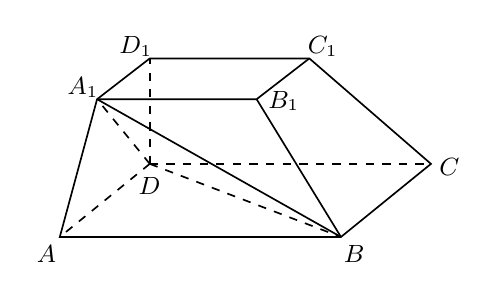
\begin{tikzpicture}[x=0.035cm, y=0.035cm, >=stealth, semithick, font=\small]
  % ===== 顶点 =====
  \coordinate (A)  at (0,0);
  \coordinate (B)  at (102.01,0);
  \coordinate (C)  at (134.66,26.52);
  \coordinate (D)  at (32.64,26.52);
  \coordinate (A1) at (13.52,49.98);
  \coordinate (B1) at (71.41,49.98);
  \coordinate (C1) at (90.54,64.78);
  \coordinate (D1) at (32.64,64.78);

  % ===== 可见的棱（实线） =====
  \draw (A) -- (B) -- (C) -- (C1) -- (D1) -- (A1) -- cycle;
  \draw (A1) -- (B1) -- (C1);
  \draw (B1) -- (B);
  \draw (A1) -- (B);

  % ===== 被遮挡的棱（虚线） =====
  \draw[dashed] (D) -- (A);
  \draw[dashed] (D) -- (C);
  \draw[dashed] (D) -- (B);
  \draw[dashed] (D) -- (A1);
  \draw[dashed] (D) -- (D1);

  % ===== 顶点标记（位置取原页字形盒中心）=====
  \node at (27.57,69.00) {$D_1$};
  \node at (8.42,54.20) {$A_1$};
  \node at (81.27,49.30) {$B_1$};
  \node at (95.37,69.00) {$C_1$};
  \node at (141.37,25.45) {$C$};
  \node at (32.57,18.45) {$D$};
  \node at (-4.83,-6.05) {$A$};
  \node at (106.82,-6.05) {$B$};
\end{tikzpicture}
\end{center}
\nopagebreak[4]
\Needspace{4\baselineskip}
\textbf{解析}

\Needspace{5\baselineskip}
设 $AD=a$，则 $AB=2a$。因为 $ABCD-A_1B_1C_1D_1$ 是棱台，上、下底面相似且对应边互相平行，相似比
\nopagebreak[4]
\[
\frac{A_1B_1}{AB}=\frac{AD}{2AD}=\frac12,
\]
故 $A_1D_1\parallel AD$、$A_1C_1\parallel AC$，且 $A_1C_1=\dfrac12AC$。又 $D_1D\perp$ 平面 $ABCD$，故 $D_1D$ 垂直于底面内的每一条直线，特别 $D_1D\perp AD$、$D_1D\perp BD$。

\gksubpart{(1)}

\Needspace{5\baselineskip}
在 $\triangle ABD$ 中，$AB=2a$、$AD=a$、$\angle BAD=60^\circ$，由余弦定理
\nopagebreak[4]
\[
BD^2=a^2+(2a)^2-2\cdot a\cdot2a\cdot\cos60^\circ=5a^2-2a^2=3a^2,
\]
\Needspace{5\baselineskip}
故 $BD=\sqrt3\,a$。于是
\nopagebreak[4]
\[
AD^2+BD^2=a^2+3a^2=4a^2=AB^2,
\]
由勾股定理的逆定理得 $\angle ADB=90^\circ$，即 $AD\perp BD$。

\Needspace{5\baselineskip}
$BD\perp AD$，$BD\perp D_1D$，而 $AD$ 与 $D_1D$ 是平面 $ADD_1A_1$ 内过 $D$ 的两条相交直线，由线面垂直的判定定理，
\nopagebreak[4]
\[
BD\perp\ \text{\text{平面}}\ ADD_1A_1.
\]
$AA_1\subset$ 平面 $ADD_1A_1$，由线面垂直的性质得 $BD\perp AA_1$，即 $AA_1\perp BD$。

\Needspace{5\baselineskip}
代数复核：取 $a=2$，$A(0,0,0)$、$D(2,0,0)$，并把 $\overrightarrow{AB}$（长 $4$、与 $AD$ 成 $60^\circ$）放在 $xOy$ 平面内，得 $B\left(4\cos60^\circ,4\sin60^\circ,0\right)=(2,2\sqrt3,0)$。则
\nopagebreak[4]
\[
\overrightarrow{BD}=D-B=(0,-2\sqrt3,0),\qquad |BD|=2\sqrt3=\sqrt3\,a\ ,
\]
且 $\overrightarrow{AD}=(2,0,0)$、$\overrightarrow{AD}\cdot\overrightarrow{BD}=0$，故 $AD\perp BD$ 。

\Needspace{5\baselineskip}
设 $D_1=(2,0,h)$（$DD_1$ 竖直），上底与下底相似比 $\dfrac12$ 给出 $A_1=\left(1,0,h\right)$，故 $\overrightarrow{AA_1}=(1,0,h)$：
\nopagebreak[4]
\[
\overrightarrow{BD}\cdot\overrightarrow{AA_1}=0\times1+(-2\sqrt3)\times0+0\times h=0\ ,
\]
即 $AA_1\perp BD$，与几何论证一致。

\gksubpart{(2)}

取 $N$ 为 $AC$ 与 $BD$ 的交点。底面 $ABCD$ 是平行四边形，对角线互相平分，故 $N$ 是 $AC$ 的中点，$N\in BD$。

\Needspace{5\baselineskip}
由 (1) 前的相似关系 $A_1C_1\parallel AC$ 且
\nopagebreak[4]
\[
A_1C_1=\frac12AC=NC,
\]
\Needspace{5\baselineskip}
四边形 $A_1C_1CN$ 有一组对边平行且相等，是平行四边形，故
\nopagebreak[4]
\[
A_1N\parallel CC_1.
\]
又 $A_1N\subset$ 平面 $A_1BD$（$A_1$ 与 $N$ 都在该平面内，$N$ 在 $BD$ 上）。

再说明 $C\notin$ 平面 $A_1BD$。平面 $A_1BD$ 与底面 $ABCD$ 的交线是 $BD$（两点 $B$、$D$ 都在底面上，故交线就是直线 $BD$）；而 $C$ 是平行四边形 $ABCD$ 的顶点，不在对角线 $BD$ 上，故 $C\notin$ 平面 $A_1BD$。

由线面平行的判定定理（平面外一条直线与平面内一条直线平行，则该直线与平面平行），$CC_1\parallel$ 平面 $A_1BD$。

代数复核：取 $a=2$、$h=1$，$A(0,0,0)$、$B(2,2\sqrt3,0)$、$C(4,2\sqrt3,0)$、$D(2,0,0)$，$A_1(1,0,1)$、$C_1(3,\sqrt3,1)$。$N$ 为 $AC$ 中点 $(2,\sqrt3,0)$，恰在 $BD$（$B(2,2\sqrt3,0)$ 到 $D(2,0,0)$ 的竖直线段）上 。$\overrightarrow{A_1N}=(1,\sqrt3,-1)$，$\overrightarrow{CC_1}=C_1-C=(-1,-\sqrt3,1)=-\overrightarrow{A_1N}$ ，两者平行反向。平面 $A_1BD$ 内 $\overrightarrow{BD}=(0,-2\sqrt3,0)$、$\overrightarrow{BA_1}=(-1,-2\sqrt3,1)$，法向量取 $\boldsymbol n=\overrightarrow{BD}\times\overrightarrow{BA_1}=(-2\sqrt3\cdot1-0\cdot(-2\sqrt3),\ 0\cdot(-1)-0\cdot1,\ 0\cdot(-2\sqrt3)-(-2\sqrt3)(-1))=(-2\sqrt3,0,-2\sqrt3)$，化简为 $(1,0,1)$。则 $\boldsymbol n\cdot\overrightarrow{CC_1}=1\times(-1)+0+1\times1=0$ ，且 $\boldsymbol n\cdot(C-A_1)=(1,0,1)\cdot(3,2\sqrt3,0)=3\neq0$，确认 $C$ 不在平面内 。

\gkanswer{答案（1）：证明见解析。}

\gkanswer{答案（2）：证明见解析。}

\end{answer}
\begin{answer}
\gksolhead{20}{}

\textbf{题目}：

等比数列 $\{a_n\}$ 中，$a_1$，$a_2$，$a_3$ 分别是下表第一、二、三行中的某一个数，且 $a_1$，$a_2$，$a_3$ 中的任何两个数不在下表的同一列。

\begin{center}
\begin{tabular}{llll}
\toprule
 & 第一列 & 第二列 & 第三列 \\
\midrule
第一行 & $3$ & $2$ & $10$ \\
第二行 & $6$ & $4$ & $14$ \\
第三行 & $9$ & $8$ & $18$ \\
\bottomrule
\end{tabular}
\end{center}

（1） 求数列 $\{a_n\}$ 的通项公式；

（2） 若数列 $\{b_n\}$ 满足：$b_n=a_n+(-1)^n\ln a_n$，求数列 $\{b_n\}$ 的前 $2n$ 项和 $S_{2n}$。

\Needspace{4\baselineskip}
\textbf{解析}

\gksubpart{(1)}

\Needspace{5\baselineskip}
三行三列的数分别为
\nopagebreak[4]
\[
\begin{array}{c|ccc}
& \text{\text{第一列}} & \text{\text{第二列}} & \text{\text{第三列}}\\ \hline
\text{\text{第一行}} & 3 & 2 & 10\\
\text{\text{第二行}} & 6 & 4 & 14\\
\text{\text{第三行}} & 9 & 8 & 18
\end{array}
\]
且三数两两不同列。按 $a_1$ 的取值逐个枚举。

$a_1$ 只能取第一行的数 $3$、$2$、$10$（分别在列 $1$、$2$、$3$），$a_2$ 只能取第二行的数，$a_3$ 只能取第三行的数，且三者所在列两两不同、$a_2^2=a_1a_3$。逐组枚举（「列」写在该数后）：

若 $a_1=3$（列 $1$）：$a_2\in\{4(\text{\text{列}}2),\ 14(\text{\text{列}}3)\}$（$6$ 在列 $1$，与 $a_1$ 同列，舍）。

\begin{itemize}
\item $a_2=4$：$q=\dfrac43$，$a_3=3\times\dfrac{16}{9}=\dfrac{16}{3}$，不是表中数；
\item $a_2=14$：$q=\dfrac{14}{3}$，$a_3=3\times\dfrac{196}{9}=\dfrac{196}{3}$，不是表中数。
\end{itemize}

若 $a_1=10$（列 $3$）：$a_2\in\{6(\text{\text{列}}1),\ 4(\text{\text{列}}2)\}$（$14$ 在列 $3$，同列舍）。

\begin{itemize}
\item $a_2=6$：$a_3=10\times\dfrac{36}{100}=\dfrac{18}{5}$，不是表中数；
\item $a_2=4$：$a_3=10\times\dfrac{16}{100}=\dfrac85$，不是表中数。
\end{itemize}

若 $a_1=2$（列 $2$）：$a_2\in\{6(\text{\text{列}}1),\ 14(\text{\text{列}}3)\}$（$4$ 在列 $2$，同列舍）。

\begin{itemize}
\item $a_2=6$：$q=3$，$a_3=2\times9=18$，正是表中列 $3$ 的数，且 $a_1$（列 $2$）、$a_2$（列 $1$）、$a_3$（列 $3$）两两不同列 ；
\item $a_2=14$：$q=7$，$a_3=2\times49=98$，不是表中数。
\end{itemize}

\Needspace{5\baselineskip}
故唯一可能是 $a_1=2$、$a_2=6$、$a_3=18$，公比 $q=3$：

\nopagebreak[4]
\[
a_n=a_1q^{n-1}=2\cdot3^{n-1}.
\]

复算：$a_2=2\times3=6$ ，$a_3=2\times9=18$ ；三者分处第 $2$、$1$、$3$ 列，满足「任何两个数不同列」。

\gksubpart{(2)}

\Needspace{5\baselineskip}
由 $a_n=2\cdot3^{n-1}>0$ 得 $\ln a_n=\ln2+(n-1)\ln3$，于是
\nopagebreak[4]
\[
b_n=a_n+(-1)^n\left[\ln2+(n-1)\ln3\right].
\]
\Needspace{5\baselineskip}
前 $2n$ 项和拆成两部分：
\nopagebreak[4]
\[
S_{2n}=\sum_{k=1}^{2n}a_k+\ln2\sum_{k=1}^{2n}(-1)^k+\ln3\sum_{k=1}^{2n}(-1)^k(k-1).
\]
\Needspace{5\baselineskip}
第一部分是等比数列求和：
\nopagebreak[4]
\[
\sum_{k=1}^{2n}a_k=2\cdot\frac{3^{2n}-1}{3-1}=3^{2n}-1.
\]
第二部分：$(-1)^k$ 在 $k=1,2,\dots,2n$ 上正负成对，$\sum\limits_{k=1}^{2n}(-1)^k=0$。

\Needspace{5\baselineskip}
第三部分按对求和，把 $k=2j-1$ 与 $k=2j$ 配成一对（$j=1,2,\dots,n$）：
\nopagebreak[4]
\[
(-1)^{2j-1}(2j-2)+(-1)^{2j}(2j-1)=-(2j-2)+(2j-1)=1,
\]
每一对贡献 $1$，共 $n$ 对，故 $\sum\limits_{k=1}^{2n}(-1)^k(k-1)=n$。

\Needspace{5\baselineskip}
于是
\nopagebreak[4]
\[
S_{2n}=3^{2n}-1+n\ln3.
\]

代回验证 $n=1$：$S_2=b_1+b_2=\left(2-\ln2\right)+\left(6+\ln6\right)=8+\ln3$（因 $\ln6-\ln2=\ln3$），而公式给 $3^2-1+1\cdot\ln3=8+\ln3$ 。

\Needspace{5\baselineskip}
再验 $n=2$：$b_1=2-\ln2$，$b_2=6+\ln6$，$b_3=18-\ln18$，$b_4=54+\ln54$，和
\nopagebreak[4]
\[
80+\left(\ln6-\ln2\right)+\left(\ln54-\ln18\right)=80+\ln3+\ln3=80+2\ln3,
\]
公式给 $3^4-1+2\ln3=80+2\ln3$ 。

\gkanswer{答案（1）：$a_n=2\cdot3^{n-1}$。}

\gkanswer{答案（2）：$S_{2n}=3^{2n}-1+n\ln3$。}

\end{answer}
\begin{answer}
\gksolhead{21}{}

\textbf{题目}：

某企业拟建造如图所示的容器（不计厚度，长度单位：米），其中容器的中间为圆柱形，左右两端均为半球形，按照设计要求容器的容积为 $\dfrac{80\pi}{3}$ 立方米，且 $l\geqslant 2r$。假设该容器的建造费用仅与其表面积有关。已知圆柱形部分每平方米建造费用为 $3$ 千元，半球形部分每平方米建造费用为 $c$（$c>3$）千元。设该容器的建造费用为 $y$ 千元。

（1） 写出 $y$ 关于 $r$ 的函数表达式，并求该函数的定义域；

（2） 求该容器的建造费用最小时的 $r$。
\nopagebreak[4]
\begin{center}% 2011 年山东卷文科第 21 题：两端半球、中间圆柱的容器。
% 来源 PDF：普通高考/2011/2011山东文.pdf，SHA-256 bf61cf7bb39a3ccfc57735cd2a7ab34387cbfa6bc86a5e7f8246e13292b0e023。
% 原页：第 2 页（A3 三栏）第 2 栏下部，书页码 692。
% 重绘依据：按原页矢量层实测复刻。坐标取原页 pt：X = x_页 − 605.70，Y = 623.38 − y_页。
%   圆柱段：上下母线 y=56.67 与 y=0，左右两端面在 x=0 与 x=141.68（端面为虚线半椭圆，长半轴 14.17 已被
%   外轮廓遮去一半，只画朝内的一半，照原页）；两个半球各以端面为赤道圆，半径 28.34，圆心在母线中点；
%   半球轮廓为实线椭圆弧（上、下半弧各一），左右对称。
%   虚线：两端面竖直直径（x=0、141.68 处 y=0…56.67），两端面的内侧半椭圆，
%   以及 y=28.34 处的水平点划线（半径 r 的标注线，两端各伸到半球外缘）。
%   标注：l 的双箭头在 y=63.76 处、自 x=3.58 到 138.09；两端的 r 标注各两条（竖直直径上、下半与
%   水平半径），文字位置照原页字形盒中心。原页不画剖面线。
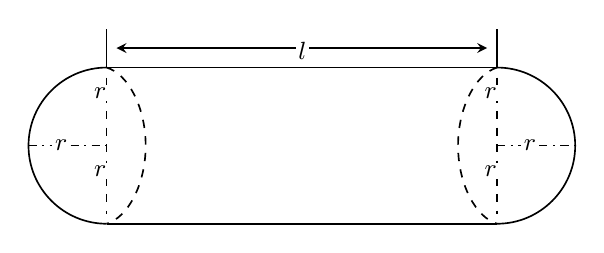
\begin{tikzpicture}[x=0.035cm, y=0.035cm, >=stealth, semithick, font=\small]

  % ===== 半球轮廓（上、下半弧，实线） =====
  \draw (0,56.67) .. controls (-15.60,56.67) and (-28.34,43.94) .. (-28.34,28.34)
        .. controls (-28.34,12.74) and (-15.60,0) .. (0,0);
  \draw (141.68,56.67) .. controls (157.28,56.67) and (170.01,43.94) .. (170.01,28.34)
        .. controls (170.01,12.74) and (157.28,0) .. (141.68,0);

  % ===== 圆柱母线（实线） =====
  \draw (0,56.67) -- (141.68,56.67);
  \draw (0,0) -- (141.68,0);

  % ===== 端面的内侧半椭圆与竖直直径（虚线） =====
  \draw[dashed] (0,56.67) .. controls (7.79,54.36) and (14.17,42.27) .. (14.17,28.34)
        .. controls (14.17,14.41) and (7.79,2.31) .. (0,0);
  \draw[dashed] (141.68,56.67) .. controls (133.89,54.36) and (127.51,42.27) .. (127.51,28.34)
        .. controls (127.51,14.41) and (133.89,2.31) .. (141.68,0);
  \draw[dashed] (0,52.98) -- (0,3.70);
  \draw[dashed] (141.68,52.98) -- (141.68,3.70);

  % ===== 半径标注线（点划线，照原页） =====
  \draw[dash dot] (-28.34,28.34) -- (0,28.34);
  \draw[dash dot] (141.68,28.34) -- (170.01,28.34);

  % ===== l 的双箭头 =====
  \draw[<->] (3.58,63.76) -- (138.09,63.76);
  \draw (0,56.67) -- (0,70.84);
  \draw (141.68,56.67) -- (141.68,70.84);
  \node[fill=white, inner sep=1pt] at (71.00,62.63) {$l$};

  % ===== r 标注（每端三条：竖直半径的上、下两段与朝外的水平半径） =====
  % 原页在标注处把虚线/点划线断开，本图用白底节点遮住线条，效果相同。
  \node[fill=white, inner sep=1pt] at (-2.30,47.38) {$r$};
  \node[fill=white, inner sep=1pt] at (139.38,47.38) {$r$};
  \node[fill=white, inner sep=1pt] at (-2.30,19.08) {$r$};
  \node[fill=white, inner sep=1pt] at (139.38,19.08) {$r$};
  \node[fill=white, inner sep=1pt] at (-16.50,28.58) {$r$};
  \node[fill=white, inner sep=1pt] at (153.58,28.58) {$r$};
\end{tikzpicture}
\end{center}
\nopagebreak[4]
\Needspace{4\baselineskip}
\textbf{解析}

\Needspace{5\baselineskip}
设圆柱段长为 $l$、半球半径为 $r$。容器容积由圆柱与两个半球组成：
\nopagebreak[4]
\[
V=\pi r^2l+\frac43\pi r^3=\frac{80\pi}{3}.
\]
\Needspace{5\baselineskip}
两边除以 $\pi$：
\nopagebreak[4]
\[
r^2l+\frac43r^3=\frac{80}{3}\ \Longrightarrow\ l=\frac{80-4r^3}{3r^2}.
\]

\gksubpart{(1)}

\Needspace{5\baselineskip}
建造费用只与表面积有关。圆柱侧面积 $2\pi rl$，两个半球合成一个整球的表面 $4\pi r^2$（半球之间的接面不算表面），故
\nopagebreak[4]
\[
y=3\cdot 2\pi rl+c\cdot4\pi r^2=6\pi rl+4\pi cr^2.
\]
\Needspace{5\baselineskip}
代入 $l$：
\nopagebreak[4]
\[
y=6\pi r\cdot\frac{80-4r^3}{3r^2}+4\pi cr^2=\frac{2\pi(80-4r^3)}{r}+4\pi cr^2=\frac{160\pi}{r}-8\pi r^2+4\pi cr^2,
\]
\Needspace{5\baselineskip}
即
\nopagebreak[4]
\[
y=\frac{160\pi}{r}+4\pi(c-2)r^2.
\]
\Needspace{5\baselineskip}
定义域由 $l\geqslant2r$ 与 $r>0$ 共同确定：
\nopagebreak[4]
\[
\frac{80-4r^3}{3r^2}\geqslant2r\ \Longrightarrow\ 80-4r^3\geqslant6r^3\ \Longrightarrow\ r^3\leqslant8\ \Longrightarrow\ r\leqslant2,
\]
故定义域为 $0<r\leqslant2$。

代回验证：$r=2$ 时 $l=\dfrac{80-32}{12}=4=2r$ （$l\geqslant2r$ 取等）；$r=1$ 时 $l=\dfrac{80-4}{3}=\dfrac{76}{3}\approx25.3>2$ 。

\gksubpart{(2)}

\Needspace{5\baselineskip}
在 $0<r\leqslant2$ 上求 $y$ 的最小值：
\nopagebreak[4]
\[
y'=-\frac{160\pi}{r^2}+8\pi(c-2)r=8\pi\left[(c-2)r-\frac{20}{r^2}\right].
\]
\Needspace{5\baselineskip}
令 $y'=0$ 得
\nopagebreak[4]
\[
(c-2)r^3=20\ \Longrightarrow\ r_0=\sqrt[3]{\frac{20}{c-2}}.
\]
\Needspace{5\baselineskip}
（$c>3$ 保证 $c-2>0$，$r_0$ 存在且为正。）又
\nopagebreak[4]
\[
y''=\frac{320\pi}{r^3}+8\pi(c-2)>0,
\]
故 $r_0$ 是极小值点，也是定义域内的最小值点（若 $r_0$ 落在定义域内）。

\textbf{判断 $r_0$ 是否落在 $(0,2]$ 内}：$r_0\leqslant2\iff\dfrac{20}{c-2}\leqslant8\iff c-2\geqslant\dfrac52\iff c\geqslant\dfrac92=4.5$。

\begin{itemize}
\item 当 $3<c\leqslant4.5$ 时，$r_0\geqslant2$，即在 $(0,2]$ 上恒有 $r<r_0$，从而 $(c-2)r^3<20$、$y'<0$，$y$ 在 $(0,2]$ 上单调递减，最小值在右端点 $r=2$ 处；
\item 当 $c>4.5$ 时，$0<r_0<2$，$y$ 在 $(0,r_0)$ 上递减、在 $(r_0,2]$ 上递增，最小值在 $r=r_0=\sqrt[3]{\dfrac{20}{c-2}}$ 处。
\end{itemize}

$c=4.5$ 时 $r_0=\sqrt[3]{8}=2$，两种情形的结论一致（都在 $r=2$ 取最小），归入前一情形。

代回验证：取 $c=4$（属 $3<c\leqslant4.5$），$r_0=\sqrt[3]{10}\approx2.15>2$，$y=\dfrac{160\pi}{r}+8\pi r^2$ 在 $r=2$ 处 $y=80\pi+32\pi=112\pi$，在 $r=1.9$ 处 $y=\dfrac{160\pi}{1.9}+8\pi\times3.61\approx84.21\pi+28.88\pi=113.09\pi>112\pi$ ，端点确为最小。取 $c=6$（属 $c>4.5$），$r_0=\sqrt[3]{5}\approx1.71<2$，$y=\dfrac{160\pi}{r}+16\pi r^2$：$y(1.71)\approx93.57\pi+46.79\pi=140.36\pi$；$y(1.6)\approx100\pi+40.96\pi=140.96\pi$；$y(1.8)\approx88.89\pi+51.84\pi=140.73\pi$，内部驻点确为最小 。

\gkanswer{答案（1）：$y=\dfrac{160\pi}{r}+4\pi(c-2)r^2$，定义域 $0<r\leqslant2$。}

\gkanswer{答案（2）：当 $3<c\leqslant4.5$ 时 $r=2$；当 $c>4.5$ 时 $r=\sqrt[3]{\dfrac{20}{c-2}}$。}

\end{answer}
\begin{answer}
\gksolhead{22}{}

\textbf{题目}：

在平面直角坐标系 $xOy$ 中，已知椭圆 $C:\dfrac{x^2}{3}+y^2=1$。如图所示，斜率为 $k$（$k>0$）且不过原点的直线 $l$ 交椭圆 $C$ 于 $A$，$B$ 两点，线段 $AB$ 的中点为 $E$，射线 $OE$ 交椭圆 $C$ 于点 $G$，交直线 $x=-3$ 于点 $D(-3,m)$。

（1） 求 $m^2+k^2$ 的最小值；

（2） 若 $|OG|^2=|OD|\cdot|OE|$，

　　① 求证：直线 $l$ 过定点；

　　② 试问点 $B$，$G$ 能否关于 $x$ 轴对称？若能，求出此时 $\triangle ABG$ 的外接圆方程；若不能，请说明理由。
\nopagebreak[4]
\begin{center}% 2011 年山东卷文科第 22 题：椭圆 C、直线 l、射线 OE 与直线 x = -3。
% 来源 PDF：普通高考/2011/2011山东文.pdf，SHA-256 bf61cf7bb39a3ccfc57735cd2a7ab34387cbfa6bc86a5e7f8246e13292b0e023。
% 原页：第 2 页（A3 三栏）第 3 栏中部，书页码 692。
% 重绘依据：原页矢量层实测定标——椭圆外框 x∈[-49.08,49.08]pt、y∈[-28.34,28.34]pt，
%   半长轴∶半短轴 = 49.08∶28.34 ≈ √3∶1，与题设 x²/3+y²=1 完全一致，故取 28.34pt = 1 单位；
%   竖直直线 x=-3 在原页实测位于 -85.01pt = -3 单位，印证该定标。
%   原页要素（单位坐标）：x 轴自 -3.50 到 2.17，y 轴自 -2.00 到 2.27；
%   直线 x=-3 自 y=2.20 到 -1.80；射线 OE 与直线 l 均画到图形之外，照原页截断。
%   本图按几何自洽重排：取 l:y=0.8x+0.5（k>0、不过原点），与椭圆 x²/3+y²=1 交于
%   A(0.5583,0.9466)、B(-1.3802,-0.6042)，中点 E(-0.4110,0.1712)；
%   射线 OE 的斜率为 -0.4167，交椭圆于 G(-1.4045,0.5852)、交 x=-3 于 D(-3,1.2500)。
%   沿射线自 O 向外的次序为 E、G、D，与原页一致；l 的两端各伸出椭圆之外。
%   标注位置照原页相对格局（D 在竖线右侧上方、G 在 OE 与椭圆交点外上侧、E 在交点下方、
%   A 在右上交点外侧、B 在左下交点外侧、O 在原点右下、-3 在 x 轴下方竖线左侧、l 在右上方）。
%   全图无网格、无辅助虚线。
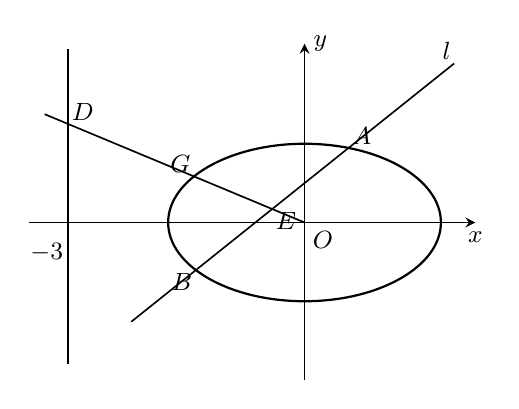
\begin{tikzpicture}[x=1cm, y=1cm, >=stealth, semithick, font=\small]

  % ===== 坐标轴 =====
  \draw[->] (-3.50,0) -- (2.17,0) node[below, inner sep=3pt] {$x$};
  \draw[->] (0,-2.00) -- (0,2.27) node[right, inner sep=3pt] {$y$};

  % ===== 椭圆 =====
  \draw[thick] (0,0) ellipse ({sqrt(3)} and 1);

  % ===== 直线 x = -3 =====
  \draw (-3,2.20) -- (-3,-1.80);

  % ===== 射线 OE（过 O、E、G、D 的直线，画到 D 之外）=====
  \draw (0,0) -- (-3.30,1.3751);
  % ===== 直线 l（过 A、B，两端伸出椭圆）=====
  \draw (-2.20,-1.2600) -- (1.90,2.0200);

  % ===== 标注 =====
  \node[above right, inner sep=1pt] at (-3,1.2500) {$D$};
  \node[above left, inner sep=1pt] at (1.90,2.0200) {$l$};
  \node[above left, inner sep=1pt] at (-1.4045,0.5852) {$G$};
  \node[above right, inner sep=1pt] at (0.5583,0.9466) {$A$};
  \node[below right, inner sep=1pt] at (-0.4110,0.1712) {$E$};
  \node[below right, inner sep=1pt] at (0.06,-0.07) {$O$};
  \node[below left, inner sep=1pt] at (-1.3802,-0.6042) {$B$};
  \node[below left, inner sep=1pt] at (-3.02,-0.22) {$-3$};

\end{tikzpicture}
\end{center}
\nopagebreak[4]
\Needspace{4\baselineskip}
\textbf{解析}

椭圆 $C:\dfrac{x^2}{3}+y^2=1$ 即 $x^2+3y^2=3$，$a=\sqrt3$、$b=1$。设 $l:y=kx+t$（$k>0$，$t\neq0$，因 $l$ 不过原点）。

\Needspace{5\baselineskip}
由 $\begin{cases}y=kx+t\\ x^2+3y^2=3\end{cases}$ 消 $y$：
\nopagebreak[4]
\[
x^2+3(kx+t)^2=3\ \Longrightarrow\ (1+3k^2)x^2+6ktx+3t^2-3=0.
\]
\Needspace{5\baselineskip}
设两根为 $x_A$、$x_B$，则
\nopagebreak[4]
\[
x_A+x_B=-\frac{6kt}{1+3k^2},\qquad x_Ax_B=\frac{3t^2-3}{1+3k^2}.
\]
\Needspace{5\baselineskip}
中点 $E$ 的横坐标 $x_E=\dfrac{x_A+x_B}{2}=-\dfrac{3kt}{1+3k^2}$，纵坐标
\nopagebreak[4]
\[
y_E=kx_E+t=-\frac{3k^2t}{1+3k^2}+t=\frac{t}{1+3k^2}.
\]
\Needspace{5\baselineskip}
故
\nopagebreak[4]
\[
k_{OE}=\frac{y_E}{x_E}=\frac{t/(1+3k^2)}{-3kt/(1+3k^2)}=-\frac{1}{3k}.
\]
点 $D(-3,m)$ 在射线 $OE$ 上，故 $m=k_{OE}\cdot(-3)=\dfrac1k$。

\gksubpart{(1)}

\nopagebreak[4]
\[
m^2+k^2=\frac{1}{k^2}+k^2\geqslant2\sqrt{\frac{1}{k^2}\cdot k^2}=2,
\]
等号当且仅当 $k^2=1$，即 $k=1$（$k>0$）。故最小值为 $2$。

代回验证：$k=1$ 时 $m=1$，$D(-3,1)$，$m^2+k^2=1+1=2$ 。

\gksubpart{(2)}

\textbf{① 求证直线 $l$ 过定点。}

沿射线 $OE$ 设点 $P=\lambda(-3k,1)$（$\lambda>0$，方向向量取 $(-3k,1)$，与 $k_{OE}=-\dfrac{1}{3k}$ 一致）。则 $|OP|=\lambda\sqrt{9k^2+1}$。

\begin{itemize}
\item 点 $E$：由 $x_E=-3k\lambda_E=-\dfrac{3kt}{1+3k^2}$ 得 $\lambda_E=\dfrac{t}{1+3k^2}$。这里要求 $t>0$：$D(-3,m)$ 在\textbf{射线} $OE$ 上（而不是 $OE$ 的反向延长线上），$x_D=-3<0$ 与 $x_E=-\dfrac{3kt}{1+3k^2}<0$ 同号，故 $t>0$。
\item 点 $D$：$x_D=-3=-3k\lambda_D$ 得 $\lambda_D=\dfrac1k$，且 $|OD|=\dfrac1k\sqrt{9k^2+1}$。
\item 点 $G$：把 $P=\lambda(-3k,1)$ 代入椭圆 $x^2+3y^2=3$：
\end{itemize}
\nopagebreak[4]
\[
9k^2\lambda^2+3\lambda^2=3\ \Longrightarrow\ \lambda_G^2=\frac{1}{3k^2+1},\qquad
\lambda_G=\frac{1}{\sqrt{3k^2+1}}.
\]
于是 $|OG|^2=\lambda_G^2(9k^2+1)=\dfrac{9k^2+1}{3k^2+1}$。

\Needspace{5\baselineskip}
条件 $|OG|^2=|OD|\cdot|OE|$ 即
\nopagebreak[4]
\[
\frac{9k^2+1}{3k^2+1}=\frac{1}{k}\sqrt{9k^2+1}\cdot\frac{t}{1+3k^2}\sqrt{9k^2+1}
=\frac{t(9k^2+1)}{k(1+3k^2)}.
\]
\Needspace{5\baselineskip}
两边约去 $\dfrac{9k^2+1}{3k^2+1}$（非零），得 $1=\dfrac tk$，即
\nopagebreak[4]
\[
t=k.
\]
故 $l:y=kx+k=k(x+1)$，直线恒过定点 $(-1,0)$。

\textbf{② 点 $B$，$G$ 能否关于 $x$ 轴对称。}

\Needspace{5\baselineskip}
设能。由 ① 知 $t=k$，$l:y=k(x+1)$。设 $B(x_B,y_B)$ 在 $l$ 与椭圆上，则 $G(x_B,-y_B)$ 在椭圆上（椭圆关于 $x$ 轴对称，自动成立），还需 $G$ 在射线 $OE$ 上，即
\nopagebreak[4]
\[
-y_B=k_{OE}\,x_B=-\frac{1}{3k}x_B\ \Longrightarrow\ y_B=\frac{x_B}{3k}.
\]
\Needspace{5\baselineskip}
把 $y_B=k(x_B+1)$ 代入：
\nopagebreak[4]
\[
\frac{x_B}{3k}=k(x_B+1)\ \Longrightarrow\ x_B=3k^2(x_B+1)\ \Longrightarrow\ x_B\left(1-3k^2\right)=3k^2\ \Longrightarrow\ x_B=\frac{3k^2}{1-3k^2}.
\]
\Needspace{5\baselineskip}
又 $B$ 在椭圆上，用 $y_B=\dfrac{x_B}{3k}$ 代入 $x^2+3y^2=3$：
\nopagebreak[4]
\[
x_B^2+\frac{x_B^2}{3k^2}=3\ \Longrightarrow\ x_B^2\cdot\frac{3k^2+1}{3k^2}=3\ \Longrightarrow\ x_B^2=\frac{9k^2}{3k^2+1}.
\]
\Needspace{5\baselineskip}
两式联立：
\nopagebreak[4]
\[
\left(\frac{3k^2}{1-3k^2}\right)^2=\frac{9k^2}{3k^2+1}
\ \Longrightarrow\ \frac{9k^4}{(1-3k^2)^2}=\frac{9k^2}{3k^2+1}
\ \Longrightarrow\ k^2(3k^2+1)=(1-3k^2)^2.
\]
\Needspace{5\baselineskip}
展开：$3k^4+k^2=1-6k^2+9k^4$，即
\nopagebreak[4]
\[
6k^4-7k^2+1=0\ \Longrightarrow\ (6k^2-1)(k^2-1)=0,
\]
故 $k^2=1$ 或 $k^2=\dfrac16$。

\Needspace{5\baselineskip}
再用「$G$ 在射线 $OE$ 上」筛除：射线 $OE$ 的方向向量为 $(-3k,1)$，$x$ 分量为负，故射线上点的横坐标必须 $<0$（除原点）。而
\nopagebreak[4]
\[
x_B=\frac{3k^2}{1-3k^2}<0\iff 1-3k^2<0\iff k^2>\frac13.
\]
$k^2=\dfrac16<\dfrac13$ 时 $x_B=3\cdot\dfrac16\div\left(1-\dfrac12\right)=\dfrac12\times2=1>0$，对应 $G(1,-y_B)$ 在 $OE$ 的反向延长线上，不合题意，舍去。故只有 $k^2=1$，$k=1$（$k>0$）。

\Needspace{5\baselineskip}
此时 $x_B=\dfrac{3}{1-3}=-\dfrac32$，$y_B=k(x_B+1)=-\dfrac12$，即
\nopagebreak[4]
\[
B\left(-\frac32,-\frac12\right),\qquad G\left(-\frac32,\frac12\right).
\]
$A$ 是 $l$ 与椭圆的另一交点：解 $x^2+3(x+1)^2=3$，即 $4x^2+6x=0$，得 $x=0$ 或 $x=-\dfrac32$，故 $A(0,1)$。

\Needspace{5\baselineskip}
三角形 $ABG$ 的三顶点为 $A(0,1)$、$B\left(-\dfrac32,-\dfrac12\right)$、$G\left(-\dfrac32,\dfrac12\right)$。$B$、$G$ 关于 $x$ 轴对称，故 $BG$ 的垂直平分线是 $x$ 轴，外接圆圆心在 $x$ 轴上，设圆心 $(u,0)$。由 $|(u,0)-A|=|(u,0)-B|$：
\nopagebreak[4]
\[
u^2+1=\left(u+\frac32\right)^2+\frac14=u^2+3u+\frac94+\frac14=u^2+3u+\frac52,
\]
\Needspace{5\baselineskip}
得 $1=3u+\dfrac52$，即 $u=-\dfrac12$。半径平方
\nopagebreak[4]
\[
R^2=u^2+1=\frac14+1=\frac54.
\]
\Needspace{5\baselineskip}
故 $\triangle ABG$ 的外接圆方程为
\nopagebreak[4]
\[
\left(x+\frac12\right)^2+y^2=\frac54.
\]

代回验证：圆心 $\left(-\dfrac12,0\right)$ 到 $A(0,1)$ 的距离平方 $\dfrac14+1=\dfrac54$ ；到 $B\left(-\dfrac32,-\dfrac12\right)$ 的距离平方 $1+\dfrac14=\dfrac54$ ；到 $G\left(-\dfrac32,\dfrac12\right)$ 同样 $\dfrac54$ 。再验 $A$、$B$、$G$ 都在椭圆上：$A$：$0+3=3$ ；$B$：$\dfrac94+3\times\dfrac14=3$ ；$G$ 同 $B$ 。且 $G\left(-\dfrac32,\dfrac12\right)$ 在射线 $OE$（斜率 $-\dfrac13$）上：$\dfrac{1/2}{-3/2}=-\dfrac13$ ，对应 $E$ 为 $AB$ 中点 $\left(-\dfrac34,\dfrac14\right)$，$\dfrac{1/4}{-3/4}=-\dfrac13$ 。

结论：点 $B$，$G$ 能关于 $x$ 轴对称，此时 $\triangle ABG$ 的外接圆方程为 $\left(x+\dfrac12\right)^2+y^2=\dfrac54$。

\gkanswer{答案（1）：$2$。}

\gkanswer{答案（2）：① 直线 $l$ 过定点 $(-1,0)$；② 点 $B$，$G$ 能关于 $x$ 轴对称，此时 $\triangle ABG$ 的外接圆方程为 $\left(x+\dfrac12\right)^2+y^2=\dfrac54$。}

\end{answer}